
\section{Structural Analysis}
Given that barrier forming problems studied in this work are NP-hard, a natural algorithmic choice for addressing the challenge is through exploring  mathematical programming.
%
To that end, a model must be built that selects from candidate barriers, which in turn requires the construction of a representative set of barrier candidates, a rather non-trivial task. 
%
The set of candidate barriers should satisfy two conflicting constraints: (1) it should contain a minimum set line segments that achieves the desired separation and (2) its size should not be too big that it will cripple the barrier selection process. 
%
Through careful structural analysis, we notice that the barriers to be considered can be limited to \emph{tangent} or \emph{bitangent} line segments. A tangent line segment, with respect to an object or an obstacle, is a line that passes through a vertex or an edge of the object/obstacle but does not intersect its interior. A bitangent is a line segment that is tangent to two objects and/or obstacles. 
%
This allows us to significantly reduce the number of candidates to be examined at the later selection stage.

\begin{theorem}\label{theorem:sin_tan}
For any $k$ sets of polygonal or point objects $S_1, \dots, S_k$ in the workspace $\mathcal W$, the set of line segments that are tangential to the objects and obstacles contains a set of minimum cardinality that separates $S_1, \dots, S_k$. 
\end{theorem}


\begin{proof}

% We prove that there exists a set of lines with minimum cardinality that separates $S_1, \dots, S_k$, and consists of only lines tangent to object vertices. 
Consider a set of line segments $L^*$ with minimum cardinality that separates $S_1,\dots, S_k$. 
Without loss of generality, we assume all line segments in $L^*$ do not end in the free space, i.e., each line segment in $L^*$ ends
at either object boundaries or workspace boundaries.
If some line segment in a minimum barrier is not tangent to any object vertex, denoted it as $\ell=OA$ (shown in Fig.~\ref{fig:proof}), we show that it can be replaced by a line segment that is tangent to some object vertex. 
%
Fix one end of $\ell$, $O$ in this case, and rotate $\ell$ around $O$ in both clockwise and counterclockwise directions until it hits some object vertex and becomes tangential to the object.
%
Denote the two line segments resulting from clockwise rotation and counterclockwise rotation as $\ell_1'=OB$ and $\ell'_2=OC$, respectively. 

We show $\ell$ can be replaced with $\ell_1'$ or $\ell_2'$. 
If this is not the case,
since replacing $\ell$ with $\ell_1'$ cannot make the separation work, there must be some point $P_1$ between $AB$ that is path connected to some point in the other class without crossing any line segments in $L^*$ when $\ell$ is replaced with $\ell'_1$. Denote the point as $D_1$ and the path as $path_1$. 
The same analysis goes for $\ell'_2$, that if $\ell$ cannot be replaced by $\ell_2$ then there is some point $P_2$ in $AC$ and path $path_2$ that connects $P_2$ to some other point $D_2$ in a different class and crosses segment $\ell$ but not $\ell_2'$. 
Since there are no objects or obstacles inside triangle $OCB$, we can assume the parts of $path_1$ and $path_2$ inside triangle $OCB$ are straight lines.
So, $path_1$ and $path_2$ must cross each other at some point. 
Denote the cross point as $Q\in path_1 \cap path_2$. 
Then, $path_1 = path_{11} (from\ P_1\ to\ Q) + path_{12} (from\ Q\ to\ D_1)$ and $path_2 = path_{12} (from\ P_2\ to\ Q) + path_{22} (from\ Q\ to\ D_2)$. 
Path $p_{11} + p_{22}$ connects $P_1$ to $D_2$, and $p_{21} + p_{12}$ connects $P_2$ to $D_1$, one of which must not cross $\ell$. 
This leads to a contradiction to the fact that the original line set $L^*$ separates the $k$ classes of objects.

Therefore, each non-tangent line segment in $L^*$ can be replaced with a tangent line segment. 
It will eventually result in a set of tangent barriers with minimum cardinality that separates $S_1,\dots,S_k$.
\begin{figure}[ht]
    \vspace{-2mm}
    \centering
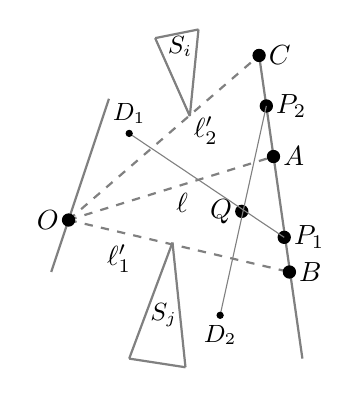
\begin{tikzpicture}[scale = 1.1]
\draw[gray, thick] (0.1, 0) -- (0.7666, 2);
\draw[gray, thick] (3, -1) -- (2.5, 2.5);


\draw[gray, thick] (1, -1) -- (1.5, 0.34);
\draw[gray, thick] (1.65, -1.1) -- (1.5, 0.34);
\draw[gray, thick] (1.65, -1.1) -- (1, -1);

\draw[gray, thick] (1.3, 2.7) -- (1.7, 1.8);
\draw[gray, thick] (1.8, 2.8) -- (1.7, 1.8);
\draw[gray, thick] (1.8, 2.8) -- (1.3, 2.7);

\draw[gray, thick, dashed] (0.3, 0.6) -- (2.66666, 1.333);

\draw[gray, thick, dashed] (0.3, 0.6) -- (2.5, 2.5);
\draw[gray, thick, dashed] (0.3, 0.6) -- (2.85, 0);

\node[text width=1cm] at (2, 0.8) {$\ell$};
\node[text width=1cm] at (2.2, 1.63) {$\ell_2'$};
\node[text width=1cm] at (1.2, 0.15) {$\ell_1'$};

\filldraw[black] (0.3, 0.6) circle (2pt) node[anchor=east] {$O$};
\filldraw[black] (2.666, 1.333) circle (2pt) node[anchor=west] {$A$};
\filldraw[black] (2.5, 2.5) circle (2pt) node[anchor=west] {$C$};
\filldraw[black] (2.85, 0) circle (2pt) node[anchor=west] {$B$};

\filldraw[black] (2.79, 0.4) circle (2pt) node[anchor=west] {$P_1$};
\filldraw[black] (2.5833, 1.917) circle (2pt) node[anchor=west] {$P_2$};

\filldraw[black] (2.3, 0.7) circle (2pt) node[anchor=east] {$Q$};

\draw[gray] (2.79, 0.4) -- (1.0, 1.6);
\draw[gray] (2.5833, 1.917) -- (2.05, -0.5);
\filldraw[black] (1.0, 1.6) circle (1pt) node[anchor=south] {\small{$D_1$}};
\filldraw[black] (2.05, -0.5) circle (1pt) node[anchor=north] {\small $D_2$};


\node[text width=1cm] at (1.9, 2.6) {\small $S_i$};
\node[text width=1cm] at (1.7, -0.5) {\small $S_j$};

\end{tikzpicture}
    \caption{Rotating non-tangent barrier line segment $\ell$ in clockwise and counterclockwise directions around its endpoint $O$ until it becomes tangential to some objects.}
    \label{fig:proof}
    \vspace{-2mm}
\end{figure}
% Then, we show that there exists a set of lines with minimum cardinality that separates $S1$ and $S2$. Similarly, when a line is only tangent to one vertex
\end{proof}

Although we can limit the candidate barriers to line segments tangent to object vertices, there can
still be infinite number of candidates. 
One may consider using line segments that are bitangent to
object vertices, i.e. line segments crossing two object or obstacle vertices. If there are $n$ object/obstacle vertices, there can be at most $n^2$, i.e., a quadratic number of bitangents. 
Unfortunately, bitangent lines are insufficient to act as candidate barriers by themselves for polygonal objects. A counterexample in Fig.~\ref{fig:counter} shows that there is an instance where an optimal solution must contain line segments that are not bitangents. 
%
In this counterexample, we need separate the orange objects from the lime object. A minimum of three line segments are used, and it is not possible that all of them are bitangent, i.e.

\begin{proposition}
Bitangent line segments do not always contain optimal solution for the barrier forming problem for polygonal objects.
\end{proposition}

\begin{figure}[ht]
    \centering
    \vspace{-.2in}
    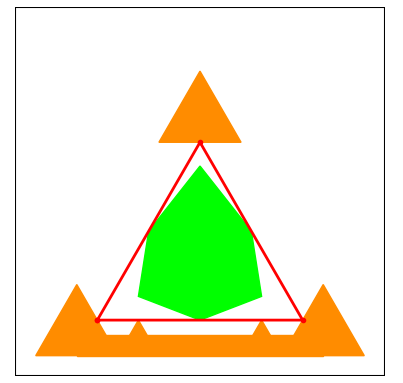
\includegraphics[width = .25\textwidth]{chapters/bc/fig/counter_example.png}
    \vspace{0.0in}
    \caption{Counterexample that shows using only bitangent line segments cannot create the optimal solution}
    \label{fig:counter}
\end{figure}

Despite the caveat, for the first two formulations that deal with barrier forming for point sets, even with polygonal obstacles, bitangent line segments
always contain an optimal solution. More precisely, 
\begin{theorem}
For any $k$ sets of point objects $S_1, \dots, S_k$ in a workspace $\mathcal W$, there exists
a set of line segments with minimum cardinality that separates $S_1, \dots, S_k$, 
and only consists of bitangent line segments.
\end{theorem}

\begin{proof}
From Theorem~\ref{theorem:sin_tan}, we can see using single tangent line segments is always enough
for an optimal solution. 
Now we turn an optimal solution, $L^*$, with only tangent line segments, into
a solution with only bitangent line segments while still maintaining the same number of barriers. 

For a tangent line segment $\ell=AB\in L^*$ with tangent point $O$ (shown in Fig.~\ref{fig:proof_bi}), and if $O$ is a point object, assume it is beneath $\ell$,
rotate $\ell$ clockwise around $O$ until it hits a point object or an obstacle vertex.
Denote the resulting line segment as $\ell'$, and replace $\ell$ with $\ell'$.
Since the objects are point objects, so $BB'$ and $AA'$ must belong to obstacles or workspace boundary, 
and thus there is no object point inside $OAA'$ or $OBB'$. 
Therefore, the replacement won't result in
any path connecting objects in different classes.
If this is not the case, then there will be some path connecting two object points in different classes that crosses $\ell$ but does not cross $\ell'$ or other barriers. 
Since the triangle areas $OAA'$ and $OBB'$ are empty, that path must enter region $OAA'$ or $OBB'$ and leave them from $\ell$. Then, that part of the path could be replaced with a straight line segment parallel to $\ell$ which prevents it from crossing $\ell$. This contradicts the assumption that $L^*$ prevents all connections between objects in different classes. % of objects.

Continuing the replacement until all line segments are bitangent will result in an optimal solution with only bitangent line segments.

\begin{figure}[ht]
    \centering
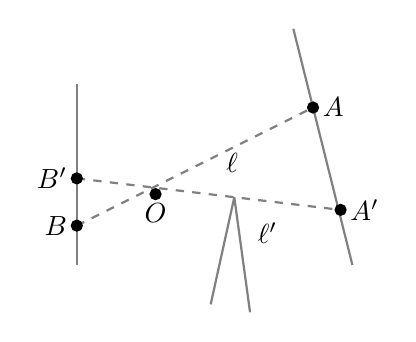
\begin{tikzpicture}
% \draw[gray, thick] (0, 0) -- (1, 2);
\draw[gray, thick] (2.5, -1) -- (1.75, 2);
\draw[gray, thick] (-1, -1) -- (-1, 1.3);

\draw[gray, thick] (0.7, -1.5) -- (1, -0.14);
\draw[gray, thick] (1.2, -1.6) -- (1, -0.14);

% \draw[gray, thick] (3, -1) -- (2.5, 2.5);

% \draw[gray, thick] (1, -1) -- (1.5, 0.34);
% \draw[gray, thick] (1.65, -1.1) -- (1.5, 0.34);
% 
% \draw[gray, thick, dashed] (0.3, 0.6) -- (2.66666, 1.333);
\draw[gray, thick, dashed] (-1., -0.5) -- (2., 1.);

\draw[gray, thick, dashed] (-1., 0.1) -- (2.35, -0.3);

% \draw[gray, thick, dashed] (0.3, 0.6) -- (2.5, 2.5);
% \draw[gray, thick, dashed] (0.3, 0.6) -- (2.85, 0);

\node[text width=1cm] at (1.4, 0.3) 
                        {$\ell$};
% \node[text] at (1.8, 1.63) 
                        % {$\ell_2'$};
\node[text width=1cm] at (1.8, -0.6) 
                        {$\ell'$};

\filldraw[black] (0.0, -0.1) circle (2pt) node[anchor=north] {$O$};
\filldraw[black] (2, 1.) circle (2pt) node[anchor=west] {$A$};
% \filldraw[black] (2.5, 2.5) circle (2pt) node[anchor=west] {$C$};
\filldraw[black] (-1, -0.5) circle (2pt) node[anchor=east] {$B$};

\filldraw[black] (2.35, -0.3) circle (2pt) node[anchor=west] {$A'$};
\filldraw[black] (-1, 0.1) circle (2pt) node[anchor=east] {$B'$};

% \filldraw[black] (2.7583, 0.6666) circle (2pt) node[anchor=west] {$P_1$};
% \filldraw[black] (2.5833, 1.917) circle (2pt) node[anchor=west] {$P_2$};

\end{tikzpicture}
    \caption{Rotating a single tangent barrier line segment $\ell$ around its tangent point $O$ clockwise until it becomes bitangent.}
    \label{fig:proof_bi}
\end{figure}
\end{proof}

For separating polygonal objects, although using bitangent line segments cannot guarantee an optimal solution that uses minimum number of line segments, they can still ensure that solutions limited to bitangents are at least $2$-optimal.
\begin{proposition}
For any $k$ sets of polygonal objects $S_1, \dots, S_k$ in the workspace $\mathcal W$, there exists a set of line segments with cardinality at most twice the minimum cardinality, that separates $S_1, \dots, S_k$, and only consists of line segments that are bitangent to object or obstacle vertices. 
\end{proposition}
\begin{proof}


\begin{figure}[ht]
    \centering
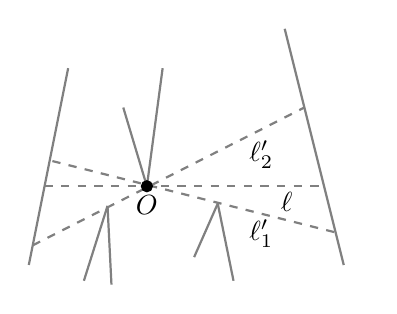
\begin{tikzpicture}

\draw[gray, thick] (2.5, -1) -- (1.75, 2);
\draw[gray, thick] (-1.5, -1) -- (-1, 1.5);
\draw[gray, thick] (0, 0) -- (-0.3, 1);
\draw[gray, thick] (0, 0) -- (.2, 1.5);

\draw[gray, thick] (-0.8, -1.2) -- (-0.5, -0.25);
\draw[gray, thick] (-0.45, -1.25) -- (-0.5, -0.25);

\draw[gray, thick] (0.6, -0.9) -- (0.9, -0.22);
\draw[gray, thick] (1.1, -1.2) -- (0.9, -0.22);


\draw[gray, thick, dashed] (-1.45, -0.75) -- (2., 1.);
\draw[gray, thick, dashed] (-1.3, -0.0) -- (2.2, 0);

\draw[gray, thick, dashed] (-1.2, 0.32) -- (2.45, -0.6);



\node[text width=1cm] at (2.2, -0.2) 
                        {$\ell$};

\node[text width=1cm] at (1.8, -0.6) 
                        {$\ell'_1$};

\node[text width=1cm] at (1.8, 0.4) 
                        {$\ell'_2$};

\filldraw[black] (0.0, -0.0) circle (2pt) node[anchor=north] {$O$};


\end{tikzpicture}
    \caption{Rotating tangent barrier line segment $\ell$ both clockwise and counterclockwise around its tangent point $O$ until it becomes bitangent.}
    \label{fig:proof_bi_2opt}
\end{figure}

Starting from an optimal solution $L^*$ with only tangent line segments,
we will replace each tangent line segment with two bitangent line segments.

Rotate each non-bitangent line segment $\ell\in L^*$ around its tangent point $O$ in clockwise or counterclockwise directions until the line segment become bitangent, as illustrated in Fig.~\ref{fig:proof_bi_2opt}. 
Since any path connecting two objects in different classes and is cut by barrier $\ell$ will still be cut by $\ell'_1$ and $\ell'_2$.
The replacement can still guarantee the separation among the object groups.
After replacing all barriers, we can obtain a 2-OPT solution with the number of line segments twice the minimum.
\end{proof}
